\section{Top-down syntax analysis}

\subsection*{ELL(1) method}
A grammar $G$ represented as a machine net is ELL(1) if: 
\begin{itemize}
    \item It does not have any leftmost recursive derivations. 
    \item Its pilot graph satisfies the ELR(1) condition. 
    \item Its pilot graph does not have any multiple transitions (single transition property). 
\end{itemize}

The ELL(1) condition above implies that the family of the ELL(1) grammars is contained in that of the ELR(1) grammars.
Furthermore, also the family of ELL(1) languages is strictly contained in that of the ELR(1) languages: 
\[\textnormal{ELL(1)} \subset \textnormal{ELR(1)}\]
\begin{example}
    Consider the grammar: 
    \[
    \begin{cases}
        E \rightarrow T^{*} \\
        T \rightarrow '('E')'|a
    \end{cases}
    \]
    The pilot is ELR(1) as found before, it has the single transition property.
    Furthermore, it has no left recursion.
    As a result the grammar is also ELL(1).
\end{example}
The ELL(1) analysis is more simple than the ELR(1). 
The main properties are: 
\begin{itemize}
    \item Predictive decision since we have only one item in each m-state base. 
        As a result we know immediately which rule to apply. 
    \item Stack pointer unnecessary once the rule to be applied is known. 
        As a result we don't need to carry on more than one analysis thread, and it is unnecessary to keep the items corresponding to other analysis hypotheses.
    \item Contraction of the stack because we have only one analysis thread. 
        As a result we don't need to push on stack the state path followed, and it suffices to push on stack the sequence of machines followed. 
    \item Simplification of the pilot: m-states with same kernel are unified (unify look-ahead).
        Transitions with same label from kernel-identical m-states go into kernel-identical m-states
        The m-state bases (with non-initial states) contain only one item (consequence of STP); thus, they are in a one-to-one correspondence with the non-initial states of the machine net. 
\end{itemize}
\begin{example}
    Consider the grammar: 
    \[
    \begin{cases}
        E \rightarrow T^{*} \\
        T \rightarrow '('E')'|a
    \end{cases}
    \]
    We have shown that it is both ELR(1) and ELL(1), so we can construct the simplified version of the pilot which is: 
    \begin{figure}[H]
        \centering
        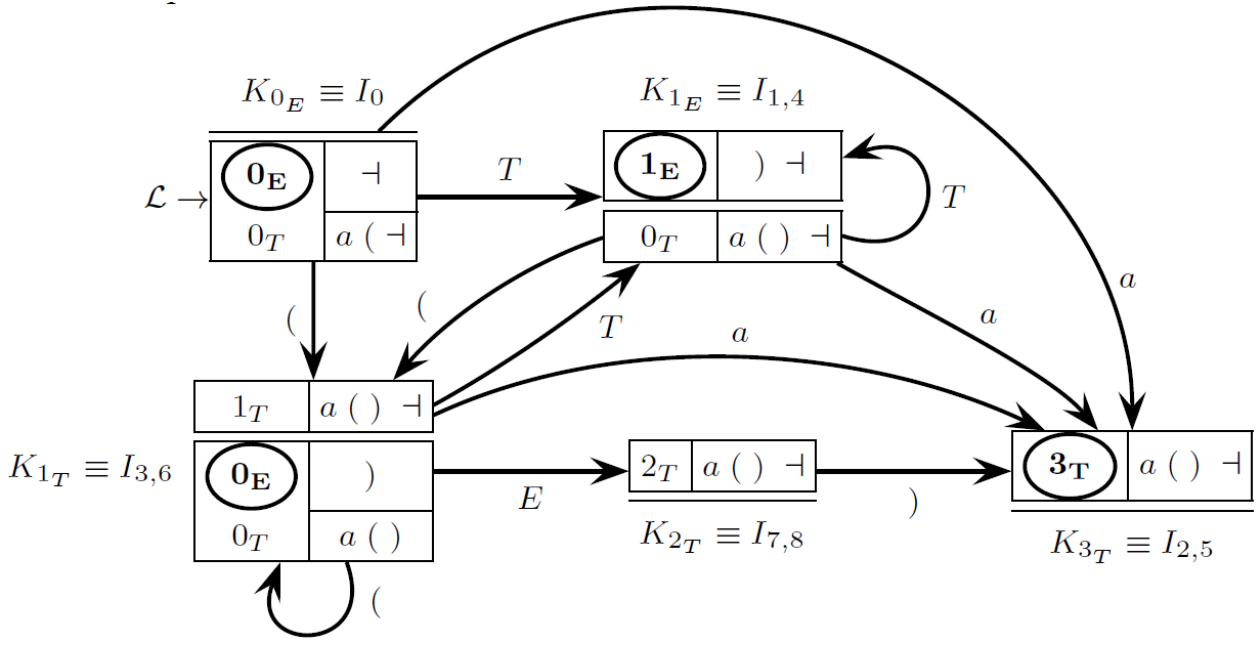
\includegraphics[width=0.6\linewidth]{images/pil1.png}
    \end{figure}
\end{example}

\subsection*{Parser control-flow graph}
The parser control-flow graph (PCFG) is the control unit of the ELL(1) syntax analyzer. 
The prospect sets are included only in the final states to choose whether to exit the machine or to continue with some more moves. 
The call arcs are dashed and labeled with a guide set, that is the set of characters that are expected in the input soon after calling the machine. 
The guide set allows choosing whether: 
\begin{itemize}
    \item Executing one call move. 
    \item Scanning a terminal symbol. 
    \item Executing one of two or more call moves. 
    \item Exiting the machine (if final state).
\end{itemize}
\begin{example}
    Consider the pilot of the previous example. 
    The corresponding parser control-flow graph is as follows: 
    \begin{figure}[H]
        \centering
        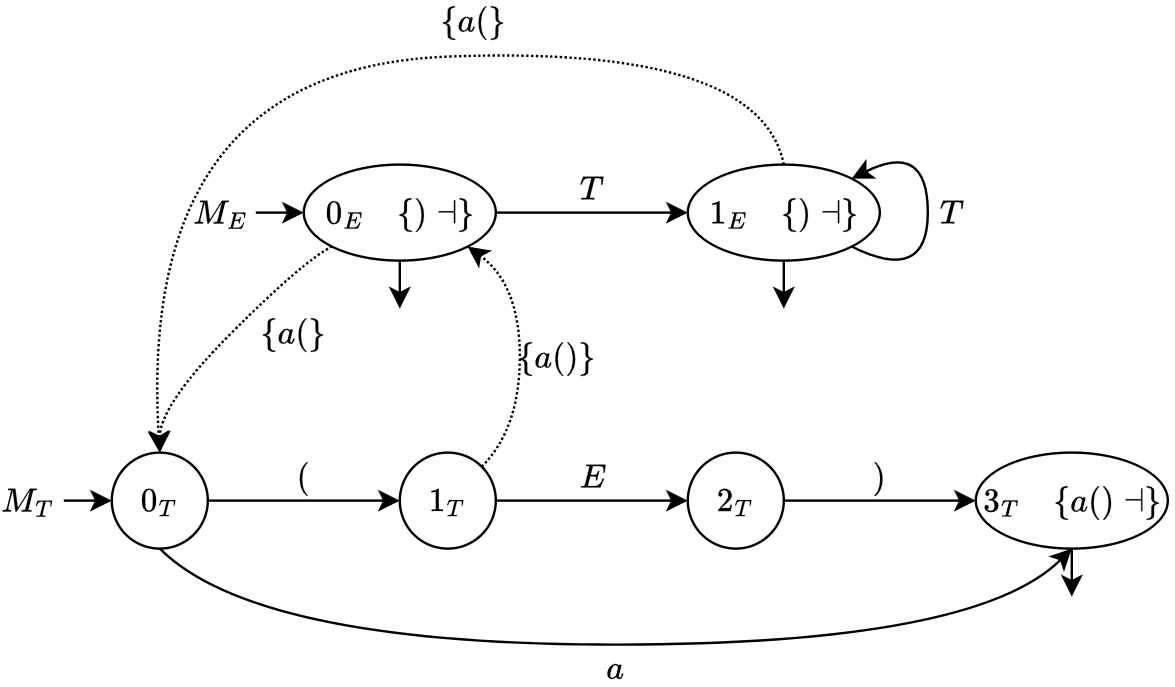
\includegraphics[width=0.6\linewidth]{images/pcfg.png}
    \end{figure}
\end{example}

The character $b$ is in the guide set, denoted as $b \in \textnormal{Gui}(q_A \dashrightarrow 0_{A_1})$, if one of the following properties holds:  
\begin{itemize}
    \item $b \in \textnormal{Ini}(L(0_{A_1}))$. 
    \item $A_1$ is nullable and $b \in \textnormal{Ini}(L(r_A))$. 
    \item $A_1$ and $L(r_A)$ are both nullable and $b \in \pi_{r_A}$.
    \item Exists in $\mathcal{F}$ a call arc $0_{A_1} \overset{\gamma_2}{\dashrightarrow} 0_{A_2}$ and $b \in \gamma_2$. 
\end{itemize}
The guide sets of the call arcs that depart from the same state have to be disjoint from one another, and be disjoint from all the scan arcs from the same state. 

In a PCFG almost all the arcs (except the non-terminal shift) are interpreted as conditional instructions: 
\begin{itemize}
    \item Terminal arcs $p \overset{a}{\rightarrow} q$ run if an only if the current character $cc=a$. 
    \item Call arcs $q_A \rightarrow 0_B$ run if an only if the current character is $cc \in \textnormal{Gui}(q_A \rightarrow 0_B)$. 
    \item Exit arcs (darts) $f_A \rightarrow$ from a state with an item $\left\langle f_A, \pi \right\rangle$ run if and only if the current character is $cc \in \pi$. 
    \item The non-terminal arcs $p \overset{a}{\rightarrow} q$ are interpreted as (unconditioned) return instructions from a machine. 
\end{itemize}
\begin{property}
    If the guide sets are disjoint, then the condition for ELL(1) is satisfied. 
\end{property}

\subsection*{Algorithm}
The stack elements are the states of the PCFG. 
The stack is initialized with element $\left\langle 0_E \right\rangle$. 
Suppose $\left\langle q_A \right\rangle$ is the stack top (it means that machine $M$, is active and in the state $q_A$). 
The ELL syntax analyzer has four move types: 
\begin{itemize}
    \item Scan move: if the shift arc $q_A \overset{cc}{\rightarrow}r_A$ exists, then scan the next token and replace the stack top by $\left\langle r_A \right\rangle$ (the active machine does not change). 
    \item Call move: if there exists a call arc $q_A \overset{\gamma}{\dashrightarrow} 0_B$ such that $cc \in \gamma$, let $q_A \overset{B}{\rightarrow}r_A$ be the corresponding nonterminal shift arc; then pop, push element $\left\langle r_A \right\rangle$ and push element $\left\langle 0_B \right\rangle$.
    \item Return move: if $q_A$ is a final state and token $cc$ is in the prospect set associated with $q_A$, then pop. 
    \item Recognition move: if $M_A$ is the axiom machine, $q_A$ is a final state and $cc =\dashv$, then accept and halt. 
\end{itemize}
In any other case the analyzer stops and rejects the input string.

\subsection*{Parser implementation by means of recursive procedures}
With this implementation the machine becomes a procedure without parameters and, consequently, we have  one procedure per each nonterminal. 
A call move become a procedure call, a can move become a call procedure next, and a return move become a return from procedure. 
Parser Control Flow Graph becomes the control graph of the procedure. 

Use the guide sets and the prospect sets to choose which move to execute. 
The analysis starts by calling the axiomatic procedure. 

\subsection*{Direct construction of the parser control-flow graph}
It is possible to construct the PCFG without building the full ELR pilot graph. 
To do this we simply put call arcs on the machine net and annotate the net with the prospect and guide sets. 

To build the prospect set we have to distinguish between initial states and other states. 
For the initial states $0_A$ we have that: 
\[\pi_{0_A}:=\pi_{0_A} \cup \bigcup_{q_i \overset{A}{\rightarrow} r_i}\left( \textnormal{Ini}(L(r_i)) \cup \textnormal{ if Null}(L(r_i)) \textnormal{ then } \pi_{q_i} \textnormal{ else } \varnothing \right)\]
For every non-initial state we have: 
\[\pi_q:=\bigcup_{p_i \overset{X_i}{\rightarrow}q}\pi_{p_i}\]

To build the guide set we have to apply iteratively this formula: 
\[\textnormal{Gui}(q_A \dashrightarrow 0_{A_1}):=\bigcup
\begin{cases}
    \textnormal{Ini}(L(A_1)) \\
    \textnormal{If Null}(A_1) \textnormal{ then Ini}(L(r_A)) \textnormal{ else } \varnothing \\
    \textnormal{If Null}(A_1) \land \textnormal{Null}(L(r_A)) \textnormal{ then Ini}(\pi_(r_A)) \textnormal{ else } \varnothing \\
    \bigcup_{0_{A_1} \dashrightarrow 0_{B_i}}\textnormal{Gui}(0_{A_1} \dashrightarrow 0_{B_i})
\end{cases}\]
Furthermore (for the final darts and the terminal shift arcs): 
\[\textnormal{Gui}(f_A \rightarrow):=\pi_{f_A}\]
\[\textnormal{Gui}(q_A \overset{a}{\rightarrow}r_A):=\{a\}\]

\subsection*{Modification of grammar not in ELL(1)}
If the ELL(1) condition is not verified, we can try to modify the grammar and make it of type ELL(1).
This approach may take a long time and be a hard work. 

The alternative approach consists in using a longer look-ahead: the analyzer looks at a number $k >1$ of consecutive characters in the input. 
If the guide sets of length $k$ on alternative moves are disjoint, then the ELL(k) analysis is possible.